%
% i0slide.tex
%
% (c) 2020 Prof Dr Andreas Müller, Hochschule Rapperswil
%
\bgroup

\def\iJ{
    \draw[color=red,line width=1.5pt] 
(4.2930,3.1186)
	-- (4.3375,3.2914)
	-- (4.3820,3.4185)
	-- (4.4265,3.5187)
	-- (4.4710,3.6020)
	-- (4.5155,3.6736)
	-- (4.5600,3.7364)
	-- (4.6045,3.7924)
	-- (4.6490,3.8429)
	-- (4.6935,3.8888)
	-- (4.7380,3.9309)
	-- (4.7825,3.9697)
	-- (4.8270,4.0056)
	-- (4.8715,4.0391)
	-- (4.9160,4.0704)
	-- (4.9605,4.0997)
	-- (5.0050,4.1272)
	-- (5.0495,4.1532)
	-- (5.0940,4.1777)
	-- (5.1385,4.2010)
	-- (5.1830,4.2231)
	-- (5.2275,4.2440)
	-- (5.2720,4.2640)
	-- (5.3165,4.2831)
	-- (5.3610,4.3013)
	-- (5.4055,4.3187)
	-- (5.4500,4.3354)
	-- (5.4945,4.3513)
	-- (5.5390,4.3667)
	-- (5.5835,4.3814)
	-- (5.6280,4.3956)
	-- (5.6725,4.4092)
	-- (5.7170,4.4224)
	-- (5.7615,4.4350)
	-- (5.8060,4.4473)
	-- (5.8505,4.4591)
	-- (5.8950,4.4705)
	-- (5.9395,4.4815)
	-- (5.9840,4.4922)
	-- (6.0285,4.5025)
	-- (6.0730,4.5125)
	-- (6.1175,4.5222)
	-- (6.1620,4.5317)
	-- (6.2065,4.5408)
	-- (6.2510,4.5497)
	-- (6.2955,4.5583)
	-- (6.3400,4.5667)
	-- (6.3845,4.5748)
	-- (6.4290,4.5827)
	-- (6.4735,4.5904)
	-- (6.5180,4.5979)
	-- (6.5625,4.6053)
	-- (6.6070,4.6124)
	-- (6.6515,4.6193)
	-- (6.6960,4.6261)
	-- (6.7405,4.6327)
	-- (6.7850,4.6391)
	-- (6.8295,4.6454)
	-- (6.8740,4.6516)
	-- (6.9185,4.6575)
	-- (6.9630,4.6634)
	-- (7.0075,4.6691)
	-- (7.0520,4.6747)
	-- (7.0965,4.6802)
	-- (7.1410,4.6855)
	-- (7.1855,4.6908)
	-- (7.2300,4.6959)
	-- (7.2745,4.7009)
	-- (7.3190,4.7058)
	-- (7.3635,4.7106)
	-- (7.4080,4.7153)
	-- (7.4525,4.7199)
	-- (7.4970,4.7244)
	-- (7.5415,4.7289)
	-- (7.5860,4.7332)
	-- (7.6305,4.7375)
	-- (7.6750,4.7416)
	-- (7.7195,4.7457)
	-- (7.7640,4.7497)
	-- (7.8085,4.7537)
	-- (7.8530,4.7576)
	-- (7.8975,4.7613)
	-- (7.9420,4.7651)
	-- (7.9865,4.7687)
	-- (8.0310,4.7723)
	-- (8.0755,4.7759)
	-- (8.1200,4.7793)
	-- (8.1645,4.7828)
	-- (8.2090,4.7861)
	-- (8.2535,4.7894)
	-- (8.2980,4.7926)
	-- (8.3425,4.7958)
	-- (8.3870,4.7990)
	-- (8.4315,4.8020)
	-- (8.4760,4.8051)
	-- (8.5205,4.8081)
	-- (8.5650,4.8110)
	-- (8.6095,4.8139)
	-- (8.6540,4.8167)
	-- (8.6985,4.8195)
	-- (8.7430,4.8223)
	-- (8.7875,4.8250)
	-- (8.8320,4.8277)
	-- (8.8765,4.8303)
	-- (8.9210,4.8329)
	-- (8.9655,4.8354)
	-- (9.0100,4.8379)
	-- (9.0545,4.8404)
	-- (9.0990,4.8429)
	-- (9.1435,4.8453)
	-- (9.1880,4.8476)
	-- (9.2325,4.8500)
	-- (9.2770,4.8523)
	-- (9.3215,4.8546)
	-- (9.3660,4.8568)
	-- (9.4105,4.8590)
	-- (9.4550,4.8612)
	-- (9.4995,4.8633)
	-- (9.5440,4.8655)
	-- (9.5885,4.8675)
	-- (9.6330,4.8696)
	-- (9.6775,4.8716)
	-- (9.7220,4.8737)
	-- (9.7665,4.8756)
	-- (9.8110,4.8776)
	-- (9.8555,4.8795)
	-- (9.9000,4.8814);
}
\def\iK{
    \draw[color=red,line width=1.5pt] 
(4.6935,1.9979)
	-- (4.7380,2.7311)
	-- (4.7825,2.8393)
	-- (4.8270,2.9379)
	-- (4.8715,3.0191)
	-- (4.9160,3.0879)
	-- (4.9605,3.1478)
	-- (5.0050,3.2009)
	-- (5.0495,3.2485)
	-- (5.0940,3.2918)
	-- (5.1385,3.3313)
	-- (5.1830,3.3678)
	-- (5.2275,3.4015)
	-- (5.2720,3.4329)
	-- (5.3165,3.4622)
	-- (5.3610,3.4897)
	-- (5.4055,3.5155)
	-- (5.4500,3.5398)
	-- (5.4945,3.5629)
	-- (5.5390,3.5847)
	-- (5.5835,3.6054)
	-- (5.6280,3.6251)
	-- (5.6725,3.6438)
	-- (5.7170,3.6617)
	-- (5.7615,3.6788)
	-- (5.8060,3.6952)
	-- (5.8505,3.7109)
	-- (5.8950,3.7259)
	-- (5.9395,3.7403)
	-- (5.9840,3.7542)
	-- (6.0285,3.7676)
	-- (6.0730,3.7804)
	-- (6.1175,3.7928)
	-- (6.1620,3.8048)
	-- (6.2065,3.8164)
	-- (6.2510,3.8275)
	-- (6.2955,3.8383)
	-- (6.3400,3.8487)
	-- (6.3845,3.8588)
	-- (6.4290,3.8686)
	-- (6.4735,3.8781)
	-- (6.5180,3.8873)
	-- (6.5625,3.8962)
	-- (6.6070,3.9049)
	-- (6.6515,3.9133)
	-- (6.6960,3.9215)
	-- (6.7405,3.9295)
	-- (6.7850,3.9372)
	-- (6.8295,3.9447)
	-- (6.8740,3.9521)
	-- (6.9185,3.9592)
	-- (6.9630,3.9662)
	-- (7.0075,3.9730)
	-- (7.0520,3.9796)
	-- (7.0965,3.9860)
	-- (7.1410,3.9923)
	-- (7.1855,3.9984)
	-- (7.2300,4.0044)
	-- (7.2745,4.0103)
	-- (7.3190,4.0160)
	-- (7.3635,4.0216)
	-- (7.4080,4.0271)
	-- (7.4525,4.0324)
	-- (7.4970,4.0377)
	-- (7.5415,4.0428)
	-- (7.5860,4.0478)
	-- (7.6305,4.0527)
	-- (7.6750,4.0575)
	-- (7.7195,4.0622)
	-- (7.7640,4.0668)
	-- (7.8085,4.0713)
	-- (7.8530,4.0757)
	-- (7.8975,4.0800)
	-- (7.9420,4.0843)
	-- (7.9865,4.0885)
	-- (8.0310,4.0925)
	-- (8.0755,4.0966)
	-- (8.1200,4.1005)
	-- (8.1645,4.1043)
	-- (8.2090,4.1081)
	-- (8.2535,4.1118)
	-- (8.2980,4.1155)
	-- (8.3425,4.1191)
	-- (8.3870,4.1226)
	-- (8.4315,4.1261)
	-- (8.4760,4.1295)
	-- (8.5205,4.1328)
	-- (8.5650,4.1361)
	-- (8.6095,4.1393)
	-- (8.6540,4.1425)
	-- (8.6985,4.1456)
	-- (8.7430,4.1487)
	-- (8.7875,4.1517)
	-- (8.8320,4.1547)
	-- (8.8765,4.1576)
	-- (8.9210,4.1605)
	-- (8.9655,4.1633)
	-- (9.0100,4.1661)
	-- (9.0545,4.1689)
	-- (9.0990,4.1716)
	-- (9.1435,4.1742)
	-- (9.1880,4.1768)
	-- (9.2325,4.1794)
	-- (9.2770,4.1820)
	-- (9.3215,4.1845)
	-- (9.3660,4.1869)
	-- (9.4105,4.1894)
	-- (9.4550,4.1918)
	-- (9.4995,4.1941)
	-- (9.5440,4.1965)
	-- (9.5885,4.1988)
	-- (9.6330,4.2010)
	-- (9.6775,4.2033)
	-- (9.7220,4.2055)
	-- (9.7665,4.2076)
	-- (9.8110,4.2098)
	-- (9.8555,4.2119)
	-- (9.9000,4.2140);
}
\def\iL{
    \draw[color=red,line width=1.5pt] 
(5.1385,1.5493)
	-- (5.1830,2.3643)
	-- (5.2275,2.4545)
	-- (5.2720,2.5353)
	-- (5.3165,2.6021)
	-- (5.3610,2.6599)
	-- (5.4055,2.7107)
	-- (5.4500,2.7562)
	-- (5.4945,2.7973)
	-- (5.5390,2.8348)
	-- (5.5835,2.8692)
	-- (5.6280,2.9011)
	-- (5.6725,2.9307)
	-- (5.7170,2.9584)
	-- (5.7615,2.9843)
	-- (5.8060,3.0086)
	-- (5.8505,3.0316)
	-- (5.8950,3.0533)
	-- (5.9395,3.0738)
	-- (5.9840,3.0934)
	-- (6.0285,3.1119)
	-- (6.0730,3.1296)
	-- (6.1175,3.1465)
	-- (6.1620,3.1626)
	-- (6.2065,3.1781)
	-- (6.2510,3.1929)
	-- (6.2955,3.2071)
	-- (6.3400,3.2208)
	-- (6.3845,3.2339)
	-- (6.4290,3.2465)
	-- (6.4735,3.2587)
	-- (6.5180,3.2704)
	-- (6.5625,3.2818)
	-- (6.6070,3.2927)
	-- (6.6515,3.3033)
	-- (6.6960,3.3135)
	-- (6.7405,3.3234)
	-- (6.7850,3.3330)
	-- (6.8295,3.3423)
	-- (6.8740,3.3513)
	-- (6.9185,3.3601)
	-- (6.9630,3.3686)
	-- (7.0075,3.3768)
	-- (7.0520,3.3848)
	-- (7.0965,3.3926)
	-- (7.1410,3.4002)
	-- (7.1855,3.4076)
	-- (7.2300,3.4147)
	-- (7.2745,3.4217)
	-- (7.3190,3.4285)
	-- (7.3635,3.4352)
	-- (7.4080,3.4416)
	-- (7.4525,3.4480)
	-- (7.4970,3.4541)
	-- (7.5415,3.4601)
	-- (7.5860,3.4660)
	-- (7.6305,3.4717)
	-- (7.6750,3.4773)
	-- (7.7195,3.4828)
	-- (7.7640,3.4882)
	-- (7.8085,3.4934)
	-- (7.8530,3.4985)
	-- (7.8975,3.5035)
	-- (7.9420,3.5084)
	-- (7.9865,3.5132)
	-- (8.0310,3.5179)
	-- (8.0755,3.5225)
	-- (8.1200,3.5270)
	-- (8.1645,3.5315)
	-- (8.2090,3.5358)
	-- (8.2535,3.5400)
	-- (8.2980,3.5442)
	-- (8.3425,3.5483)
	-- (8.3870,3.5523)
	-- (8.4315,3.5562)
	-- (8.4760,3.5601)
	-- (8.5205,3.5638)
	-- (8.5650,3.5676)
	-- (8.6095,3.5712)
	-- (8.6540,3.5748)
	-- (8.6985,3.5783)
	-- (8.7430,3.5818)
	-- (8.7875,3.5852)
	-- (8.8320,3.5885)
	-- (8.8765,3.5918)
	-- (8.9210,3.5950)
	-- (8.9655,3.5982)
	-- (9.0100,3.6013)
	-- (9.0545,3.6043)
	-- (9.0990,3.6074)
	-- (9.1435,3.6103)
	-- (9.1880,3.6132)
	-- (9.2325,3.6161)
	-- (9.2770,3.6189)
	-- (9.3215,3.6217)
	-- (9.3660,3.6244)
	-- (9.4105,3.6271)
	-- (9.4550,3.6298)
	-- (9.4995,3.6324)
	-- (9.5440,3.6350)
	-- (9.5885,3.6375)
	-- (9.6330,3.6400)
	-- (9.6775,3.6425)
	-- (9.7220,3.6449)
	-- (9.7665,3.6473)
	-- (9.8110,3.6496)
	-- (9.8555,3.6520)
	-- (9.9000,3.6543);
}
\def\iM{
    \draw[color=red,line width=1.5pt] 
(5.5390,1.4554)
	-- (5.5835,1.9367)
	-- (5.6280,2.0508)
	-- (5.6725,2.1259)
	-- (5.7170,2.1924)
	-- (5.7615,2.2489)
	-- (5.8060,2.2981)
	-- (5.8505,2.3418)
	-- (5.8950,2.3811)
	-- (5.9395,2.4169)
	-- (5.9840,2.4497)
	-- (6.0285,2.4800)
	-- (6.0730,2.5082)
	-- (6.1175,2.5344)
	-- (6.1620,2.5590)
	-- (6.2065,2.5820)
	-- (6.2510,2.6038)
	-- (6.2955,2.6243)
	-- (6.3400,2.6438)
	-- (6.3845,2.6623)
	-- (6.4290,2.6799)
	-- (6.4735,2.6966)
	-- (6.5180,2.7126)
	-- (6.5625,2.7279)
	-- (6.6070,2.7426)
	-- (6.6515,2.7566)
	-- (6.6960,2.7701)
	-- (6.7405,2.7831)
	-- (6.7850,2.7955)
	-- (6.8295,2.8075)
	-- (6.8740,2.8191)
	-- (6.9185,2.8302)
	-- (6.9630,2.8410)
	-- (7.0075,2.8514)
	-- (7.0520,2.8614)
	-- (7.0965,2.8712)
	-- (7.1410,2.8806)
	-- (7.1855,2.8897)
	-- (7.2300,2.8986)
	-- (7.2745,2.9072)
	-- (7.3190,2.9155)
	-- (7.3635,2.9236)
	-- (7.4080,2.9314)
	-- (7.4525,2.9391)
	-- (7.4970,2.9465)
	-- (7.5415,2.9538)
	-- (7.5860,2.9608)
	-- (7.6305,2.9677)
	-- (7.6750,2.9743)
	-- (7.7195,2.9808)
	-- (7.7640,2.9872)
	-- (7.8085,2.9934)
	-- (7.8530,2.9994)
	-- (7.8975,3.0053)
	-- (7.9420,3.0111)
	-- (7.9865,3.0167)
	-- (8.0310,3.0222)
	-- (8.0755,3.0276)
	-- (8.1200,3.0328)
	-- (8.1645,3.0379)
	-- (8.2090,3.0430)
	-- (8.2535,3.0479)
	-- (8.2980,3.0527)
	-- (8.3425,3.0574)
	-- (8.3870,3.0620)
	-- (8.4315,3.0665)
	-- (8.4760,3.0709)
	-- (8.5205,3.0753)
	-- (8.5650,3.0795)
	-- (8.6095,3.0837)
	-- (8.6540,3.0878)
	-- (8.6985,3.0918)
	-- (8.7430,3.0957)
	-- (8.7875,3.0996)
	-- (8.8320,3.1033)
	-- (8.8765,3.1070)
	-- (8.9210,3.1107)
	-- (8.9655,3.1143)
	-- (9.0100,3.1178)
	-- (9.0545,3.1212)
	-- (9.0990,3.1246)
	-- (9.1435,3.1280)
	-- (9.1880,3.1312)
	-- (9.2325,3.1344)
	-- (9.2770,3.1376)
	-- (9.3215,3.1407)
	-- (9.3660,3.1438)
	-- (9.4105,3.1468)
	-- (9.4550,3.1497)
	-- (9.4995,3.1527)
	-- (9.5440,3.1555)
	-- (9.5885,3.1583)
	-- (9.6330,3.1611)
	-- (9.6775,3.1639)
	-- (9.7220,3.1665)
	-- (9.7665,3.1692)
	-- (9.8110,3.1718)
	-- (9.8555,3.1744)
	-- (9.9000,3.1769);
}
\def\iN{
    \draw[color=red,line width=1.5pt] 
(5.9840,1.0781)
	-- (6.0285,1.7094)
	-- (6.0730,1.7867)
	-- (6.1175,1.8469)
	-- (6.1620,1.8994)
	-- (6.2065,1.9463)
	-- (6.2510,1.9883)
	-- (6.2955,2.0262)
	-- (6.3400,2.0606)
	-- (6.3845,2.0920)
	-- (6.4290,2.1210)
	-- (6.4735,2.1479)
	-- (6.5180,2.1729)
	-- (6.5625,2.1963)
	-- (6.6070,2.2183)
	-- (6.6515,2.2390)
	-- (6.6960,2.2585)
	-- (6.7405,2.2770)
	-- (6.7850,2.2946)
	-- (6.8295,2.3113)
	-- (6.8740,2.3273)
	-- (6.9185,2.3425)
	-- (6.9630,2.3570)
	-- (7.0075,2.3710)
	-- (7.0520,2.3843)
	-- (7.0965,2.3971)
	-- (7.1410,2.4095)
	-- (7.1855,2.4213)
	-- (7.2300,2.4327)
	-- (7.2745,2.4438)
	-- (7.3190,2.4544)
	-- (7.3635,2.4646)
	-- (7.4080,2.4746)
	-- (7.4525,2.4841)
	-- (7.4970,2.4934)
	-- (7.5415,2.5024)
	-- (7.5860,2.5111)
	-- (7.6305,2.5196)
	-- (7.6750,2.5278)
	-- (7.7195,2.5357)
	-- (7.7640,2.5435)
	-- (7.8085,2.5510)
	-- (7.8530,2.5583)
	-- (7.8975,2.5654)
	-- (7.9420,2.5723)
	-- (7.9865,2.5791)
	-- (8.0310,2.5856)
	-- (8.0755,2.5920)
	-- (8.1200,2.5982)
	-- (8.1645,2.6043)
	-- (8.2090,2.6103)
	-- (8.2535,2.6161)
	-- (8.2980,2.6217)
	-- (8.3425,2.6272)
	-- (8.3870,2.6326)
	-- (8.4315,2.6379)
	-- (8.4760,2.6431)
	-- (8.5205,2.6481)
	-- (8.5650,2.6530)
	-- (8.6095,2.6579)
	-- (8.6540,2.6626)
	-- (8.6985,2.6672)
	-- (8.7430,2.6717)
	-- (8.7875,2.6762)
	-- (8.8320,2.6805)
	-- (8.8765,2.6848)
	-- (8.9210,2.6889)
	-- (8.9655,2.6930)
	-- (9.0100,2.6970)
	-- (9.0545,2.7010)
	-- (9.0990,2.7048)
	-- (9.1435,2.7086)
	-- (9.1880,2.7123)
	-- (9.2325,2.7160)
	-- (9.2770,2.7195)
	-- (9.3215,2.7231)
	-- (9.3660,2.7265)
	-- (9.4105,2.7299)
	-- (9.4550,2.7332)
	-- (9.4995,2.7365)
	-- (9.5440,2.7397)
	-- (9.5885,2.7429)
	-- (9.6330,2.7460)
	-- (9.6775,2.7490)
	-- (9.7220,2.7521)
	-- (9.7665,2.7550)
	-- (9.8110,2.7579)
	-- (9.8555,2.7608)
	-- (9.9000,2.7636);
}
\def\iO{
    \draw[color=red,line width=1.5pt] 
(6.3845,1.0550)
	-- (6.4290,1.3991)
	-- (6.4735,1.4731)
	-- (6.5180,1.5385)
	-- (6.5625,1.5939)
	-- (6.6070,1.6413)
	-- (6.6515,1.6828)
	-- (6.6960,1.7200)
	-- (6.7405,1.7531)
	-- (6.7850,1.7834)
	-- (6.8295,1.8113)
	-- (6.8740,1.8371)
	-- (6.9185,1.8611)
	-- (6.9630,1.8835)
	-- (7.0075,1.9045)
	-- (7.0520,1.9243)
	-- (7.0965,1.9429)
	-- (7.1410,1.9606)
	-- (7.1855,1.9774)
	-- (7.2300,1.9934)
	-- (7.2745,2.0086)
	-- (7.3190,2.0231)
	-- (7.3635,2.0370)
	-- (7.4080,2.0503)
	-- (7.4525,2.0630)
	-- (7.4970,2.0753)
	-- (7.5415,2.0870)
	-- (7.5860,2.0983)
	-- (7.6305,2.1093)
	-- (7.6750,2.1198)
	-- (7.7195,2.1299)
	-- (7.7640,2.1397)
	-- (7.8085,2.1492)
	-- (7.8530,2.1584)
	-- (7.8975,2.1672)
	-- (7.9420,2.1758)
	-- (7.9865,2.1842)
	-- (8.0310,2.1922)
	-- (8.0755,2.2001)
	-- (8.1200,2.2077)
	-- (8.1645,2.2151)
	-- (8.2090,2.2223)
	-- (8.2535,2.2293)
	-- (8.2980,2.2361)
	-- (8.3425,2.2428)
	-- (8.3870,2.2492)
	-- (8.4315,2.2555)
	-- (8.4760,2.2617)
	-- (8.5205,2.2676)
	-- (8.5650,2.2735)
	-- (8.6095,2.2792)
	-- (8.6540,2.2847)
	-- (8.6985,2.2902)
	-- (8.7430,2.2955)
	-- (8.7875,2.3007)
	-- (8.8320,2.3057)
	-- (8.8765,2.3107)
	-- (8.9210,2.3155)
	-- (8.9655,2.3203)
	-- (9.0100,2.3249)
	-- (9.0545,2.3295)
	-- (9.0990,2.3339)
	-- (9.1435,2.3383)
	-- (9.1880,2.3425)
	-- (9.2325,2.3467)
	-- (9.2770,2.3508)
	-- (9.3215,2.3549)
	-- (9.3660,2.3588)
	-- (9.4105,2.3627)
	-- (9.4550,2.3665)
	-- (9.4995,2.3702)
	-- (9.5440,2.3738)
	-- (9.5885,2.3774)
	-- (9.6330,2.3809)
	-- (9.6775,2.3844)
	-- (9.7220,2.3878)
	-- (9.7665,2.3911)
	-- (9.8110,2.3944)
	-- (9.8555,2.3976)
	-- (9.9000,2.4008);
}
\def\iP{
    \draw[color=red,line width=1.5pt] 
(6.8295,0.7417)
	-- (6.8740,1.2212)
	-- (6.9185,1.2848)
	-- (6.9630,1.3296)
	-- (7.0075,1.3755)
	-- (7.0520,1.4173)
	-- (7.0965,1.4532)
	-- (7.1410,1.4851)
	-- (7.1855,1.5145)
	-- (7.2300,1.5415)
	-- (7.2745,1.5663)
	-- (7.3190,1.5895)
	-- (7.3635,1.6110)
	-- (7.4080,1.6312)
	-- (7.4525,1.6501)
	-- (7.4970,1.6680)
	-- (7.5415,1.6850)
	-- (7.5860,1.7011)
	-- (7.6305,1.7164)
	-- (7.6750,1.7309)
	-- (7.7195,1.7448)
	-- (7.7640,1.7581)
	-- (7.8085,1.7708)
	-- (7.8530,1.7830)
	-- (7.8975,1.7947)
	-- (7.9420,1.8060)
	-- (7.9865,1.8168)
	-- (8.0310,1.8273)
	-- (8.0755,1.8374)
	-- (8.1200,1.8471)
	-- (8.1645,1.8565)
	-- (8.2090,1.8655)
	-- (8.2535,1.8743)
	-- (8.2980,1.8828)
	-- (8.3425,1.8911)
	-- (8.3870,1.8991)
	-- (8.4315,1.9068)
	-- (8.4760,1.9143)
	-- (8.5205,1.9216)
	-- (8.5650,1.9287)
	-- (8.6095,1.9357)
	-- (8.6540,1.9424)
	-- (8.6985,1.9489)
	-- (8.7430,1.9553)
	-- (8.7875,1.9615)
	-- (8.8320,1.9675)
	-- (8.8765,1.9734)
	-- (8.9210,1.9792)
	-- (8.9655,1.9848)
	-- (9.0100,1.9903)
	-- (9.0545,1.9956)
	-- (9.0990,2.0009)
	-- (9.1435,2.0060)
	-- (9.1880,2.0110)
	-- (9.2325,2.0159)
	-- (9.2770,2.0206)
	-- (9.3215,2.0253)
	-- (9.3660,2.0299)
	-- (9.4105,2.0343)
	-- (9.4550,2.0387)
	-- (9.4995,2.0430)
	-- (9.5440,2.0472)
	-- (9.5885,2.0513)
	-- (9.6330,2.0554)
	-- (9.6775,2.0593)
	-- (9.7220,2.0632)
	-- (9.7665,2.0670)
	-- (9.8110,2.0707)
	-- (9.8555,2.0744)
	-- (9.9000,2.0780);
}
\def\iQ{
    \draw[color=red,line width=1.5pt] 
(7.2745,0.5203)
	-- (7.3635,1.0972)
	-- (7.4080,1.1408)
	-- (7.4525,1.1833)
	-- (7.4970,1.2180)
	-- (7.5415,1.2493)
	-- (7.5860,1.2785)
	-- (7.6305,1.3043)
	-- (7.6750,1.3286)
	-- (7.7195,1.3507)
	-- (7.7640,1.3716)
	-- (7.8085,1.3910)
	-- (7.8530,1.4093)
	-- (7.8975,1.4265)
	-- (7.9420,1.4428)
	-- (7.9865,1.4583)
	-- (8.0310,1.4729)
	-- (8.0755,1.4869)
	-- (8.1200,1.5003)
	-- (8.1645,1.5130)
	-- (8.2090,1.5252)
	-- (8.2535,1.5370)
	-- (8.2980,1.5482)
	-- (8.3425,1.5590)
	-- (8.3870,1.5694)
	-- (8.4315,1.5794)
	-- (8.4760,1.5891)
	-- (8.5205,1.5984)
	-- (8.5650,1.6074)
	-- (8.6095,1.6161)
	-- (8.6540,1.6246)
	-- (8.6985,1.6327)
	-- (8.7430,1.6407)
	-- (8.7875,1.6483)
	-- (8.8320,1.6558)
	-- (8.8765,1.6630)
	-- (8.9210,1.6700)
	-- (8.9655,1.6769)
	-- (9.0100,1.6835)
	-- (9.0545,1.6900)
	-- (9.0990,1.6963)
	-- (9.1435,1.7024)
	-- (9.1880,1.7084)
	-- (9.2325,1.7142)
	-- (9.2770,1.7199)
	-- (9.3215,1.7254)
	-- (9.3660,1.7308)
	-- (9.4105,1.7361)
	-- (9.4550,1.7413)
	-- (9.4995,1.7463)
	-- (9.5440,1.7512)
	-- (9.5885,1.7560)
	-- (9.6330,1.7607)
	-- (9.6775,1.7653)
	-- (9.7220,1.7698)
	-- (9.7665,1.7743)
	-- (9.8110,1.7786)
	-- (9.8555,1.7828)
	-- (9.9000,1.7869);
}
\def\iR{
    \draw[color=red,line width=1.5pt] 
(7.6750,0.4648)
	-- (7.7640,0.8838)
	-- (7.8530,0.9769)
	-- (7.8975,1.0089)
	-- (7.9420,1.0421)
	-- (7.9865,1.0686)
	-- (8.0310,1.0948)
	-- (8.0755,1.1177)
	-- (8.1200,1.1396)
	-- (8.1645,1.1595)
	-- (8.2090,1.1784)
	-- (8.2535,1.1960)
	-- (8.2980,1.2127)
	-- (8.3425,1.2284)
	-- (8.3870,1.2433)
	-- (8.4315,1.2574)
	-- (8.4760,1.2709)
	-- (8.5205,1.2837)
	-- (8.5650,1.2960)
	-- (8.6095,1.3078)
	-- (8.6540,1.3190)
	-- (8.6985,1.3299)
	-- (8.7430,1.3403)
	-- (8.7875,1.3503)
	-- (8.8320,1.3599)
	-- (8.8765,1.3692)
	-- (8.9210,1.3782)
	-- (8.9655,1.3868)
	-- (9.0100,1.3952)
	-- (9.0545,1.4033)
	-- (9.0990,1.4112)
	-- (9.1435,1.4188)
	-- (9.1880,1.4262)
	-- (9.2325,1.4334)
	-- (9.2770,1.4403)
	-- (9.3215,1.4471)
	-- (9.3660,1.4537)
	-- (9.4105,1.4601)
	-- (9.4550,1.4663)
	-- (9.4995,1.4724)
	-- (9.5440,1.4783)
	-- (9.5885,1.4840)
	-- (9.6330,1.4896)
	-- (9.6775,1.4951)
	-- (9.7220,1.5005)
	-- (9.7665,1.5057)
	-- (9.8110,1.5108)
	-- (9.8555,1.5157)
	-- (9.9000,1.5206);
}
\def\iS{
    \draw[color=red,line width=1.5pt] 
(8.1200,0.2781)
	-- (8.1645,0.1834)
	-- (8.2090,0.7538)
	-- (8.2535,0.0513)
	-- (8.2980,0.8256)
	-- (8.3425,0.8537)
	-- (8.3870,0.8831)
	-- (8.4315,0.9067)
	-- (8.4760,0.9302)
	-- (8.5205,0.9508)
	-- (8.5650,0.9706)
	-- (8.6095,0.9892)
	-- (8.6540,1.0059)
	-- (8.6985,1.0221)
	-- (8.7430,1.0372)
	-- (8.7875,1.0517)
	-- (8.8320,1.0653)
	-- (8.8765,1.0783)
	-- (8.9210,1.0907)
	-- (8.9655,1.1026)
	-- (9.0100,1.1139)
	-- (9.0545,1.1248)
	-- (9.0990,1.1352)
	-- (9.1435,1.1452)
	-- (9.1880,1.1549)
	-- (9.2325,1.1642)
	-- (9.2770,1.1731)
	-- (9.3215,1.1818)
	-- (9.3660,1.1901)
	-- (9.4105,1.1982)
	-- (9.4550,1.2060)
	-- (9.4995,1.2136)
	-- (9.5440,1.2210)
	-- (9.5885,1.2281)
	-- (9.6330,1.2350)
	-- (9.6775,1.2417)
	-- (9.7220,1.2482)
	-- (9.7665,1.2546)
	-- (9.8110,1.2608)
	-- (9.8555,1.2668)
	-- (9.9000,1.2726);
}
\def\iT{
    \draw[color=red,line width=1.5pt] 
(8.5205,0.2432)
	-- (8.5650,0.1261)
	-- (8.6095,0.0512)
	-- (8.6540,0.6176)
	-- (8.6985,-0.1047)
	-- (8.7430,0.6896)
	-- (8.8320,0.7392)
	-- (8.8765,1.2654)
	-- (8.9210,0.7818)
	-- (8.9655,0.8011)
	-- (9.0100,0.8187)
	-- (9.0545,0.8355)
	-- (9.0990,0.8513)
	-- (9.1435,0.8658)
	-- (9.1880,0.8798)
	-- (9.2325,0.8937)
	-- (9.2770,0.9056)
	-- (9.3215,0.9176)
	-- (9.3660,0.9293)
	-- (9.4105,0.9400)
	-- (9.4550,0.9505)
	-- (9.4995,0.9606)
	-- (9.5440,0.9703)
	-- (9.5885,0.9796)
	-- (9.6330,0.9886)
	-- (9.6775,0.9972)
	-- (9.7220,1.0056)
	-- (9.7665,1.0137)
	-- (9.8110,1.0215)
	-- (9.8555,1.0290)
	-- (9.9000,1.0364);
}
\def\jJ{
    \draw[color=blue,line width=1.5pt] 
(3.4475,4.4898)
	-- (3.4920,4.7225)
	-- (3.5365,4.8882)
	-- (3.5810,5.0188)
	-- (3.6255,5.1271)
	-- (3.6700,5.2197)
	-- (3.7145,5.3007)
	-- (3.7590,5.3725)
	-- (3.8035,5.4370)
	-- (3.8480,5.4953)
	-- (3.8925,5.5486)
	-- (3.9370,5.5974)
	-- (3.9815,5.6425)
	-- (4.0260,5.6844)
	-- (4.0705,5.7233)
	-- (4.1150,5.7596)
	-- (4.1595,5.7937)
	-- (4.2040,5.8257)
	-- (4.2485,5.8558)
	-- (4.2930,5.8843)
	-- (4.3375,5.9112)
	-- (4.3820,5.9367)
	-- (4.4265,5.9609)
	-- (4.4710,5.9839)
	-- (4.5155,6.0059)
	-- (4.5600,6.0268)
	-- (4.6045,6.0468)
	-- (4.6490,6.0659)
	-- (4.6935,6.0842)
	-- (4.7380,6.1017)
	-- (4.7825,6.1185)
	-- (4.8270,6.1347)
	-- (4.8715,6.1502)
	-- (4.9160,6.1652)
	-- (4.9605,6.1796)
	-- (5.0050,6.1934)
	-- (5.0495,6.2068)
	-- (5.0940,6.2197)
	-- (5.1385,6.2322)
	-- (5.1830,6.2442)
	-- (5.2275,6.2559)
	-- (5.2720,6.2672)
	-- (5.3165,6.2781)
	-- (5.3610,6.2886)
	-- (5.4055,6.2989)
	-- (5.4500,6.3088)
	-- (5.4945,6.3185)
	-- (5.5390,6.3279)
	-- (5.5835,6.3370)
	-- (5.6280,6.3458)
	-- (5.6725,6.3544)
	-- (5.7170,6.3627)
	-- (5.7615,6.3709)
	-- (5.8060,6.3788)
	-- (5.8505,6.3865)
	-- (5.8950,6.3940)
	-- (5.9395,6.4013)
	-- (5.9840,6.4085)
	-- (6.0285,6.4154)
	-- (6.0730,6.4222)
	-- (6.1175,6.4288)
	-- (6.1620,6.4353)
	-- (6.2065,6.4416)
	-- (6.2510,6.4477)
	-- (6.2955,6.4537)
	-- (6.3400,6.4596)
	-- (6.3845,6.4654)
	-- (6.4290,6.4710)
	-- (6.4735,6.4765)
	-- (6.5180,6.4819)
	-- (6.5625,6.4871)
	-- (6.6070,6.4923)
	-- (6.6515,6.4973)
	-- (6.6960,6.5023)
	-- (6.7405,6.5071)
	-- (6.7850,6.5118)
	-- (6.8295,6.5165)
	-- (6.8740,6.5210)
	-- (6.9185,6.5255)
	-- (6.9630,6.5299)
	-- (7.0075,6.5341)
	-- (7.0520,6.5384)
	-- (7.0965,6.5425)
	-- (7.1410,6.5465)
	-- (7.1855,6.5505)
	-- (7.2300,6.5544)
	-- (7.2745,6.5582)
	-- (7.3190,6.5620)
	-- (7.3635,6.5657)
	-- (7.4080,6.5693)
	-- (7.4525,6.5729)
	-- (7.4970,6.5764)
	-- (7.5415,6.5798)
	-- (7.5860,6.5832)
	-- (7.6305,6.5865)
	-- (7.6750,6.5898)
	-- (7.7195,6.5930)
	-- (7.7640,6.5962)
	-- (7.8085,6.5993)
	-- (7.8530,6.6023)
	-- (7.8975,6.6054)
	-- (7.9420,6.6083)
	-- (7.9865,6.6112)
	-- (8.0310,6.6141)
	-- (8.0755,6.6169)
	-- (8.1200,6.6197)
	-- (8.1645,6.6225)
	-- (8.2090,6.6252)
	-- (8.2535,6.6278)
	-- (8.2980,6.6304)
	-- (8.3425,6.6330)
	-- (8.3870,6.6355)
	-- (8.4315,6.6380)
	-- (8.4760,6.6405)
	-- (8.5205,6.6429)
	-- (8.5650,6.6453)
	-- (8.6095,6.6477)
	-- (8.6540,6.6500)
	-- (8.6985,6.6523)
	-- (8.7430,6.6546)
	-- (8.7875,6.6568)
	-- (8.8320,6.6590)
	-- (8.8765,6.6611)
	-- (8.9210,6.6633)
	-- (8.9655,6.6654)
	-- (9.0100,6.6675)
	-- (9.0545,6.6696)
	-- (9.0990,6.6716)
	-- (9.1435,6.6736)
	-- (9.1880,6.6755)
	-- (9.2325,6.6775)
	-- (9.2770,6.6794)
	-- (9.3215,6.6814)
	-- (9.3660,6.6833)
	-- (9.4105,6.6851)
	-- (9.4550,6.6869)
	-- (9.4995,6.6887)
	-- (9.5440,6.6905)
	-- (9.5885,6.6922)
	-- (9.6330,6.6940)
	-- (9.6775,6.6957)
	-- (9.7220,6.6974)
	-- (9.7665,6.6991)
	-- (9.8110,6.7008)
	-- (9.8555,6.7025)
	-- (9.9000,6.7041);
}
\def\jK{
    \draw[color=blue,line width=1.5pt] 
(3.5365,3.7767)
	-- (3.5810,4.0335)
	-- (3.6255,4.2060)
	-- (3.6700,4.3375)
	-- (3.7145,4.4448)
	-- (3.7590,4.5358)
	-- (3.8035,4.6148)
	-- (3.8480,4.6846)
	-- (3.8925,4.7471)
	-- (3.9370,4.8036)
	-- (3.9815,4.8551)
	-- (4.0260,4.9023)
	-- (4.0705,4.9459)
	-- (4.1150,4.9863)
	-- (4.1595,5.0238)
	-- (4.2040,5.0589)
	-- (4.2485,5.0918)
	-- (4.2930,5.1227)
	-- (4.3375,5.1518)
	-- (4.3820,5.1793)
	-- (4.4265,5.2053)
	-- (4.4710,5.2299)
	-- (4.5155,5.2534)
	-- (4.5600,5.2756)
	-- (4.6045,5.2969)
	-- (4.6490,5.3171)
	-- (4.6935,5.3365)
	-- (4.7380,5.3550)
	-- (4.7825,5.3727)
	-- (4.8270,5.3897)
	-- (4.8715,5.4060)
	-- (4.9160,5.4217)
	-- (4.9605,5.4368)
	-- (5.0050,5.4513)
	-- (5.0495,5.4653)
	-- (5.0940,5.4787)
	-- (5.1385,5.4917)
	-- (5.1830,5.5043)
	-- (5.2275,5.5164)
	-- (5.2720,5.5281)
	-- (5.3165,5.5395)
	-- (5.3610,5.5504)
	-- (5.4055,5.5611)
	-- (5.4500,5.5714)
	-- (5.4945,5.5814)
	-- (5.5390,5.5911)
	-- (5.5835,5.6005)
	-- (5.6280,5.6096)
	-- (5.6725,5.6185)
	-- (5.7170,5.6271)
	-- (5.7615,5.6355)
	-- (5.8060,5.6437)
	-- (5.8505,5.6516)
	-- (5.8950,5.6593)
	-- (5.9395,5.6669)
	-- (5.9840,5.6742)
	-- (6.0285,5.6814)
	-- (6.0730,5.6883)
	-- (6.1175,5.6952)
	-- (6.1620,5.7018)
	-- (6.2065,5.7083)
	-- (6.2510,5.7146)
	-- (6.2955,5.7208)
	-- (6.3400,5.7268)
	-- (6.3845,5.7327)
	-- (6.4290,5.7385)
	-- (6.4735,5.7441)
	-- (6.5180,5.7496)
	-- (6.5625,5.7550)
	-- (6.6070,5.7603)
	-- (6.6515,5.7654)
	-- (6.6960,5.7705)
	-- (6.7405,5.7754)
	-- (6.7850,5.7803)
	-- (6.8295,5.7850)
	-- (6.8740,5.7897)
	-- (6.9185,5.7942)
	-- (6.9630,5.7987)
	-- (7.0075,5.8031)
	-- (7.0520,5.8074)
	-- (7.0965,5.8116)
	-- (7.1410,5.8157)
	-- (7.1855,5.8198)
	-- (7.2300,5.8238)
	-- (7.2745,5.8277)
	-- (7.3190,5.8315)
	-- (7.3635,5.8353)
	-- (7.4080,5.8390)
	-- (7.4525,5.8426)
	-- (7.4970,5.8462)
	-- (7.5415,5.8497)
	-- (7.5860,5.8532)
	-- (7.6305,5.8566)
	-- (7.6750,5.8599)
	-- (7.7195,5.8632)
	-- (7.7640,5.8664)
	-- (7.8085,5.8696)
	-- (7.8530,5.8727)
	-- (7.8975,5.8757)
	-- (7.9420,5.8788)
	-- (7.9865,5.8817)
	-- (8.0310,5.8846)
	-- (8.0755,5.8875)
	-- (8.1200,5.8903)
	-- (8.1645,5.8931)
	-- (8.2090,5.8959)
	-- (8.2535,5.8986)
	-- (8.2980,5.9012)
	-- (8.3425,5.9039)
	-- (8.3870,5.9064)
	-- (8.4315,5.9090)
	-- (8.4760,5.9115)
	-- (8.5205,5.9140)
	-- (8.5650,5.9164)
	-- (8.6095,5.9188)
	-- (8.6540,5.9212)
	-- (8.6985,5.9235)
	-- (8.7430,5.9258)
	-- (8.7875,5.9281)
	-- (8.8320,5.9303)
	-- (8.8765,5.9325)
	-- (8.9210,5.9347)
	-- (8.9655,5.9368)
	-- (9.0100,5.9390)
	-- (9.0545,5.9410)
	-- (9.0990,5.9431)
	-- (9.1435,5.9451)
	-- (9.1880,5.9471)
	-- (9.2325,5.9491)
	-- (9.2770,5.9511)
	-- (9.3215,5.9530)
	-- (9.3660,5.9549)
	-- (9.4105,5.9568)
	-- (9.4550,5.9587)
	-- (9.4995,5.9605)
	-- (9.5440,5.9623)
	-- (9.5885,5.9641)
	-- (9.6330,5.9659)
	-- (9.6775,5.9676)
	-- (9.7220,5.9693)
	-- (9.7665,5.9710)
	-- (9.8110,5.9727)
	-- (9.8555,5.9744)
	-- (9.9000,5.9761);
}
\def\jL{
    \draw[color=blue,line width=1.5pt] 
(3.6255,2.7887)
	-- (3.6700,3.4473)
	-- (3.7145,3.6343)
	-- (3.7590,3.7694)
	-- (3.8035,3.8771)
	-- (3.8480,3.9673)
	-- (3.8925,4.0450)
	-- (3.9370,4.1134)
	-- (3.9815,4.1743)
	-- (4.0260,4.2293)
	-- (4.0705,4.2793)
	-- (4.1150,4.3252)
	-- (4.1595,4.3674)
	-- (4.2040,4.4065)
	-- (4.2485,4.4429)
	-- (4.2930,4.4769)
	-- (4.3375,4.5088)
	-- (4.3820,4.5387)
	-- (4.4265,4.5669)
	-- (4.4710,4.5935)
	-- (4.5155,4.6187)
	-- (4.5600,4.6426)
	-- (4.6045,4.6653)
	-- (4.6490,4.6869)
	-- (4.6935,4.7075)
	-- (4.7380,4.7271)
	-- (4.7825,4.7459)
	-- (4.8270,4.7639)
	-- (4.8715,4.7811)
	-- (4.9160,4.7976)
	-- (4.9605,4.8135)
	-- (5.0050,4.8287)
	-- (5.0495,4.8434)
	-- (5.0940,4.8575)
	-- (5.1385,4.8711)
	-- (5.1830,4.8842)
	-- (5.2275,4.8968)
	-- (5.2720,4.9091)
	-- (5.3165,4.9209)
	-- (5.3610,4.9323)
	-- (5.4055,4.9434)
	-- (5.4500,4.9541)
	-- (5.4945,4.9644)
	-- (5.5390,4.9745)
	-- (5.5835,4.9842)
	-- (5.6280,4.9937)
	-- (5.6725,5.0029)
	-- (5.7170,5.0118)
	-- (5.7615,5.0205)
	-- (5.8060,5.0289)
	-- (5.8505,5.0371)
	-- (5.8950,5.0451)
	-- (5.9395,5.0529)
	-- (5.9840,5.0604)
	-- (6.0285,5.0678)
	-- (6.0730,5.0750)
	-- (6.1175,5.0820)
	-- (6.1620,5.0888)
	-- (6.2065,5.0955)
	-- (6.2510,5.1020)
	-- (6.2955,5.1083)
	-- (6.3400,5.1145)
	-- (6.3845,5.1206)
	-- (6.4290,5.1265)
	-- (6.4735,5.1323)
	-- (6.5180,5.1379)
	-- (6.5625,5.1435)
	-- (6.6070,5.1489)
	-- (6.6515,5.1542)
	-- (6.6960,5.1593)
	-- (6.7405,5.1644)
	-- (6.7850,5.1694)
	-- (6.8295,5.1742)
	-- (6.8740,5.1790)
	-- (6.9185,5.1837)
	-- (6.9630,5.1882)
	-- (7.0075,5.1927)
	-- (7.0520,5.1971)
	-- (7.0965,5.2014)
	-- (7.1410,5.2056)
	-- (7.1855,5.2098)
	-- (7.2300,5.2139)
	-- (7.2745,5.2179)
	-- (7.3190,5.2218)
	-- (7.3635,5.2256)
	-- (7.4080,5.2294)
	-- (7.4525,5.2331)
	-- (7.4970,5.2368)
	-- (7.5415,5.2403)
	-- (7.5860,5.2439)
	-- (7.6305,5.2473)
	-- (7.6750,5.2507)
	-- (7.7195,5.2541)
	-- (7.7640,5.2573)
	-- (7.8085,5.2606)
	-- (7.8530,5.2637)
	-- (7.8975,5.2669)
	-- (7.9420,5.2699)
	-- (7.9865,5.2730)
	-- (8.0310,5.2759)
	-- (8.0755,5.2789)
	-- (8.1200,5.2817)
	-- (8.1645,5.2846)
	-- (8.2090,5.2874)
	-- (8.2535,5.2901)
	-- (8.2980,5.2928)
	-- (8.3425,5.2955)
	-- (8.3870,5.2981)
	-- (8.4315,5.3007)
	-- (8.4760,5.3033)
	-- (8.5205,5.3058)
	-- (8.5650,5.3083)
	-- (8.6095,5.3107)
	-- (8.6540,5.3131)
	-- (8.6985,5.3155)
	-- (8.7430,5.3178)
	-- (8.7875,5.3201)
	-- (8.8320,5.3224)
	-- (8.8765,5.3246)
	-- (8.9210,5.3269)
	-- (8.9655,5.3290)
	-- (9.0100,5.3312)
	-- (9.0545,5.3333)
	-- (9.0990,5.3354)
	-- (9.1435,5.3375)
	-- (9.1880,5.3395)
	-- (9.2325,5.3415)
	-- (9.2770,5.3435)
	-- (9.3215,5.3455)
	-- (9.3660,5.3474)
	-- (9.4105,5.3493)
	-- (9.4550,5.3512)
	-- (9.4995,5.3531)
	-- (9.5440,5.3549)
	-- (9.5885,5.3567)
	-- (9.6330,5.3585)
	-- (9.6775,5.3603)
	-- (9.7220,5.3620)
	-- (9.7665,5.3638)
	-- (9.8110,5.3655)
	-- (9.8555,5.3672)
	-- (9.9000,5.3688);
}
\def\jM{
    \draw[color=blue,line width=1.5pt] 
(3.7590,2.9244)
	-- (3.8035,3.1457)
	-- (3.8480,3.2859)
	-- (3.8925,3.3959)
	-- (3.9370,3.4863)
	-- (3.9815,3.5635)
	-- (4.0260,3.6310)
	-- (4.0705,3.6908)
	-- (4.1150,3.7447)
	-- (4.1595,3.7935)
	-- (4.2040,3.8382)
	-- (4.2485,3.8794)
	-- (4.2930,3.9174)
	-- (4.3375,3.9528)
	-- (4.3820,3.9859)
	-- (4.4265,4.0168)
	-- (4.4710,4.0459)
	-- (4.5155,4.0733)
	-- (4.5600,4.0991)
	-- (4.6045,4.1236)
	-- (4.6490,4.1468)
	-- (4.6935,4.1689)
	-- (4.7380,4.1899)
	-- (4.7825,4.2099)
	-- (4.8270,4.2290)
	-- (4.8715,4.2473)
	-- (4.9160,4.2648)
	-- (4.9605,4.2815)
	-- (5.0050,4.2976)
	-- (5.0495,4.3130)
	-- (5.0940,4.3279)
	-- (5.1385,4.3421)
	-- (5.1830,4.3559)
	-- (5.2275,4.3691)
	-- (5.2720,4.3819)
	-- (5.3165,4.3943)
	-- (5.3610,4.4062)
	-- (5.4055,4.4177)
	-- (5.4500,4.4289)
	-- (5.4945,4.4397)
	-- (5.5390,4.4501)
	-- (5.5835,4.4602)
	-- (5.6280,4.4701)
	-- (5.6725,4.4796)
	-- (5.7170,4.4888)
	-- (5.7615,4.4978)
	-- (5.8060,4.5065)
	-- (5.8505,4.5150)
	-- (5.8950,4.5233)
	-- (5.9395,4.5313)
	-- (5.9840,4.5391)
	-- (6.0285,4.5467)
	-- (6.0730,4.5541)
	-- (6.1175,4.5614)
	-- (6.1620,4.5684)
	-- (6.2065,4.5753)
	-- (6.2510,4.5820)
	-- (6.2955,4.5885)
	-- (6.3400,4.5949)
	-- (6.3845,4.6011)
	-- (6.4290,4.6072)
	-- (6.4735,4.6131)
	-- (6.5180,4.6189)
	-- (6.5625,4.6246)
	-- (6.6070,4.6302)
	-- (6.6515,4.6356)
	-- (6.6960,4.6409)
	-- (6.7405,4.6461)
	-- (6.7850,4.6512)
	-- (6.8295,4.6562)
	-- (6.8740,4.6610)
	-- (6.9185,4.6658)
	-- (6.9630,4.6705)
	-- (7.0075,4.6751)
	-- (7.0520,4.6796)
	-- (7.0965,4.6840)
	-- (7.1410,4.6883)
	-- (7.1855,4.6926)
	-- (7.2300,4.6967)
	-- (7.2745,4.7008)
	-- (7.3190,4.7048)
	-- (7.3635,4.7087)
	-- (7.4080,4.7126)
	-- (7.4525,4.7164)
	-- (7.4970,4.7201)
	-- (7.5415,4.7238)
	-- (7.5860,4.7274)
	-- (7.6305,4.7309)
	-- (7.6750,4.7344)
	-- (7.7195,4.7378)
	-- (7.7640,4.7411)
	-- (7.8085,4.7444)
	-- (7.8530,4.7477)
	-- (7.8975,4.7508)
	-- (7.9420,4.7540)
	-- (7.9865,4.7571)
	-- (8.0310,4.7601)
	-- (8.0755,4.7631)
	-- (8.1200,4.7660)
	-- (8.1645,4.7689)
	-- (8.2090,4.7717)
	-- (8.2535,4.7745)
	-- (8.2980,4.7773)
	-- (8.3425,4.7800)
	-- (8.3870,4.7827)
	-- (8.4315,4.7853)
	-- (8.4760,4.7879)
	-- (8.5205,4.7905)
	-- (8.5650,4.7930)
	-- (8.6095,4.7955)
	-- (8.6540,4.7979)
	-- (8.6985,4.8004)
	-- (8.7430,4.8027)
	-- (8.7875,4.8051)
	-- (8.8320,4.8074)
	-- (8.8765,4.8097)
	-- (8.9210,4.8119)
	-- (8.9655,4.8141)
	-- (9.0100,4.8163)
	-- (9.0545,4.8185)
	-- (9.0990,4.8206)
	-- (9.1435,4.8227)
	-- (9.1880,4.8248)
	-- (9.2325,4.8268)
	-- (9.2770,4.8288)
	-- (9.3215,4.8308)
	-- (9.3660,4.8328)
	-- (9.4105,4.8347)
	-- (9.4550,4.8367)
	-- (9.4995,4.8386)
	-- (9.5440,4.8404)
	-- (9.5885,4.8423)
	-- (9.6330,4.8441)
	-- (9.6775,4.8459)
	-- (9.7220,4.8477)
	-- (9.7665,4.8494)
	-- (9.8110,4.8512)
	-- (9.8555,4.8529)
	-- (9.9000,4.8546);
}
\def\jN{
    \draw[color=blue,line width=1.5pt] 
(3.8925,2.7083)
	-- (3.9370,2.8660)
	-- (3.9815,2.9808)
	-- (4.0260,3.0729)
	-- (4.0705,3.1504)
	-- (4.1150,3.2176)
	-- (4.1595,3.2768)
	-- (4.2040,3.3298)
	-- (4.2485,3.3778)
	-- (4.2930,3.4216)
	-- (4.3375,3.4619)
	-- (4.3820,3.4991)
	-- (4.4265,3.5337)
	-- (4.4710,3.5659)
	-- (4.5155,3.5961)
	-- (4.5600,3.6244)
	-- (4.6045,3.6511)
	-- (4.6490,3.6763)
	-- (4.6935,3.7002)
	-- (4.7380,3.7228)
	-- (4.7825,3.7443)
	-- (4.8270,3.7647)
	-- (4.8715,3.7842)
	-- (4.9160,3.8029)
	-- (4.9605,3.8207)
	-- (5.0050,3.8377)
	-- (5.0495,3.8541)
	-- (5.0940,3.8697)
	-- (5.1385,3.8848)
	-- (5.1830,3.8993)
	-- (5.2275,3.9132)
	-- (5.2720,3.9266)
	-- (5.3165,3.9396)
	-- (5.3610,3.9520)
	-- (5.4055,3.9641)
	-- (5.4500,3.9757)
	-- (5.4945,3.9870)
	-- (5.5390,3.9979)
	-- (5.5835,4.0085)
	-- (5.6280,4.0187)
	-- (5.6725,4.0286)
	-- (5.7170,4.0382)
	-- (5.7615,4.0475)
	-- (5.8060,4.0566)
	-- (5.8505,4.0654)
	-- (5.8950,4.0739)
	-- (5.9395,4.0822)
	-- (5.9840,4.0903)
	-- (6.0285,4.0982)
	-- (6.0730,4.1058)
	-- (6.1175,4.1133)
	-- (6.1620,4.1206)
	-- (6.2065,4.1276)
	-- (6.2510,4.1345)
	-- (6.2955,4.1413)
	-- (6.3400,4.1478)
	-- (6.3845,4.1543)
	-- (6.4290,4.1605)
	-- (6.4735,4.1666)
	-- (6.5180,4.1726)
	-- (6.5625,4.1784)
	-- (6.6070,4.1842)
	-- (6.6515,4.1897)
	-- (6.6960,4.1952)
	-- (6.7405,4.2005)
	-- (6.7850,4.2057)
	-- (6.8295,4.2109)
	-- (6.8740,4.2159)
	-- (6.9185,4.2208)
	-- (6.9630,4.2256)
	-- (7.0075,4.2303)
	-- (7.0520,4.2349)
	-- (7.0965,4.2394)
	-- (7.1410,4.2438)
	-- (7.1855,4.2482)
	-- (7.2300,4.2524)
	-- (7.2745,4.2566)
	-- (7.3190,4.2607)
	-- (7.3635,4.2647)
	-- (7.4080,4.2687)
	-- (7.4525,4.2725)
	-- (7.4970,4.2763)
	-- (7.5415,4.2801)
	-- (7.5860,4.2837)
	-- (7.6305,4.2873)
	-- (7.6750,4.2909)
	-- (7.7195,4.2944)
	-- (7.7640,4.2978)
	-- (7.8085,4.3012)
	-- (7.8530,4.3045)
	-- (7.8975,4.3077)
	-- (7.9420,4.3109)
	-- (7.9865,4.3141)
	-- (8.0310,4.3171)
	-- (8.0755,4.3202)
	-- (8.1200,4.3232)
	-- (8.1645,4.3261)
	-- (8.2090,4.3290)
	-- (8.2535,4.3319)
	-- (8.2980,4.3347)
	-- (8.3425,4.3375)
	-- (8.3870,4.3402)
	-- (8.4315,4.3429)
	-- (8.4760,4.3455)
	-- (8.5205,4.3481)
	-- (8.5650,4.3507)
	-- (8.6095,4.3532)
	-- (8.6540,4.3557)
	-- (8.6985,4.3582)
	-- (8.7430,4.3606)
	-- (8.7875,4.3630)
	-- (8.8320,4.3653)
	-- (8.8765,4.3676)
	-- (8.9210,4.3699)
	-- (8.9655,4.3722)
	-- (9.0100,4.3744)
	-- (9.0545,4.3766)
	-- (9.0990,4.3788)
	-- (9.1435,4.3809)
	-- (9.1880,4.3830)
	-- (9.2325,4.3851)
	-- (9.2770,4.3871)
	-- (9.3215,4.3892)
	-- (9.3660,4.3912)
	-- (9.4105,4.3931)
	-- (9.4550,4.3951)
	-- (9.4995,4.3970)
	-- (9.5440,4.3989)
	-- (9.5885,4.4008)
	-- (9.6330,4.4026)
	-- (9.6775,4.4045)
	-- (9.7220,4.4063)
	-- (9.7665,4.4081)
	-- (9.8110,4.4098)
	-- (9.8555,4.4116)
	-- (9.9000,4.4133);
}
\def\jO{
    \draw[color=blue,line width=1.5pt] 
(4.0260,2.5040)
	-- (4.0705,2.6166)
	-- (4.1150,2.7120)
	-- (4.1595,2.7911)
	-- (4.2040,2.8584)
	-- (4.2485,2.9176)
	-- (4.2930,2.9702)
	-- (4.3375,3.0177)
	-- (4.3820,3.0608)
	-- (4.4265,3.1004)
	-- (4.4710,3.1370)
	-- (4.5155,3.1709)
	-- (4.5600,3.2024)
	-- (4.6045,3.2320)
	-- (4.6490,3.2597)
	-- (4.6935,3.2858)
	-- (4.7380,3.3105)
	-- (4.7825,3.3338)
	-- (4.8270,3.3559)
	-- (4.8715,3.3769)
	-- (4.9160,3.3969)
	-- (4.9605,3.4159)
	-- (5.0050,3.4341)
	-- (5.0495,3.4515)
	-- (5.0940,3.4682)
	-- (5.1385,3.4841)
	-- (5.1830,3.4995)
	-- (5.2275,3.5142)
	-- (5.2720,3.5283)
	-- (5.3165,3.5420)
	-- (5.3610,3.5551)
	-- (5.4055,3.5677)
	-- (5.4500,3.5800)
	-- (5.4945,3.5918)
	-- (5.5390,3.6032)
	-- (5.5835,3.6142)
	-- (5.6280,3.6248)
	-- (5.6725,3.6352)
	-- (5.7170,3.6452)
	-- (5.7615,3.6549)
	-- (5.8060,3.6643)
	-- (5.8505,3.6734)
	-- (5.8950,3.6823)
	-- (5.9395,3.6909)
	-- (5.9840,3.6993)
	-- (6.0285,3.7075)
	-- (6.0730,3.7154)
	-- (6.1175,3.7231)
	-- (6.1620,3.7306)
	-- (6.2065,3.7380)
	-- (6.2510,3.7451)
	-- (6.2955,3.7520)
	-- (6.3400,3.7588)
	-- (6.3845,3.7654)
	-- (6.4290,3.7719)
	-- (6.4735,3.7782)
	-- (6.5180,3.7843)
	-- (6.5625,3.7904)
	-- (6.6070,3.7962)
	-- (6.6515,3.8020)
	-- (6.6960,3.8076)
	-- (6.7405,3.8131)
	-- (6.7850,3.8184)
	-- (6.8295,3.8237)
	-- (6.8740,3.8288)
	-- (6.9185,3.8338)
	-- (6.9630,3.8388)
	-- (7.0075,3.8436)
	-- (7.0520,3.8483)
	-- (7.0965,3.8530)
	-- (7.1410,3.8575)
	-- (7.1855,3.8619)
	-- (7.2300,3.8663)
	-- (7.2745,3.8706)
	-- (7.3190,3.8748)
	-- (7.3635,3.8789)
	-- (7.4080,3.8829)
	-- (7.4525,3.8869)
	-- (7.4970,3.8908)
	-- (7.5415,3.8946)
	-- (7.5860,3.8984)
	-- (7.6305,3.9021)
	-- (7.6750,3.9057)
	-- (7.7195,3.9092)
	-- (7.7640,3.9127)
	-- (7.8085,3.9162)
	-- (7.8530,3.9195)
	-- (7.8975,3.9229)
	-- (7.9420,3.9261)
	-- (7.9865,3.9293)
	-- (8.0310,3.9325)
	-- (8.0755,3.9356)
	-- (8.1200,3.9386)
	-- (8.1645,3.9417)
	-- (8.2090,3.9446)
	-- (8.2535,3.9475)
	-- (8.2980,3.9504)
	-- (8.3425,3.9532)
	-- (8.3870,3.9560)
	-- (8.4315,3.9587)
	-- (8.4760,3.9614)
	-- (8.5205,3.9641)
	-- (8.5650,3.9667)
	-- (8.6095,3.9693)
	-- (8.6540,3.9718)
	-- (8.6985,3.9743)
	-- (8.7430,3.9768)
	-- (8.7875,3.9792)
	-- (8.8320,3.9816)
	-- (8.8765,3.9840)
	-- (8.9210,3.9863)
	-- (8.9655,3.9886)
	-- (9.0100,3.9908)
	-- (9.0545,3.9931)
	-- (9.0990,3.9953)
	-- (9.1435,3.9975)
	-- (9.1880,3.9996)
	-- (9.2325,4.0017)
	-- (9.2770,4.0038)
	-- (9.3215,4.0059)
	-- (9.3660,4.0079)
	-- (9.4105,4.0099)
	-- (9.4550,4.0119)
	-- (9.4995,4.0138)
	-- (9.5440,4.0158)
	-- (9.5885,4.0177)
	-- (9.6330,4.0195)
	-- (9.6775,4.0214)
	-- (9.7220,4.0232)
	-- (9.7665,4.0251)
	-- (9.8110,4.0268)
	-- (9.8555,4.0286)
	-- (9.9000,4.0304);
}
\def\jP{
    \draw[color=blue,line width=1.5pt] 
(4.1595,2.2915)
	-- (4.2040,2.3915)
	-- (4.2485,2.4738)
	-- (4.2930,2.5425)
	-- (4.3375,2.6021)
	-- (4.3820,2.6548)
	-- (4.4265,2.7021)
	-- (4.4710,2.7449)
	-- (4.5155,2.7841)
	-- (4.5600,2.8202)
	-- (4.6045,2.8535)
	-- (4.6490,2.8846)
	-- (4.6935,2.9137)
	-- (4.7380,2.9409)
	-- (4.7825,2.9665)
	-- (4.8270,2.9907)
	-- (4.8715,3.0135)
	-- (4.9160,3.0352)
	-- (4.9605,3.0558)
	-- (5.0050,3.0754)
	-- (5.0495,3.0940)
	-- (5.0940,3.1118)
	-- (5.1385,3.1289)
	-- (5.1830,3.1452)
	-- (5.2275,3.1608)
	-- (5.2720,3.1758)
	-- (5.3165,3.1903)
	-- (5.3610,3.2041)
	-- (5.4055,3.2175)
	-- (5.4500,3.2303)
	-- (5.4945,3.2427)
	-- (5.5390,3.2547)
	-- (5.5835,3.2663)
	-- (5.6280,3.2774)
	-- (5.6725,3.2883)
	-- (5.7170,3.2987)
	-- (5.7615,3.3089)
	-- (5.8060,3.3187)
	-- (5.8505,3.3282)
	-- (5.8950,3.3374)
	-- (5.9395,3.3464)
	-- (5.9840,3.3551)
	-- (6.0285,3.3636)
	-- (6.0730,3.3718)
	-- (6.1175,3.3798)
	-- (6.1620,3.3876)
	-- (6.2065,3.3952)
	-- (6.2510,3.4026)
	-- (6.2955,3.4098)
	-- (6.3400,3.4168)
	-- (6.3845,3.4236)
	-- (6.4290,3.4303)
	-- (6.4735,3.4368)
	-- (6.5180,3.4431)
	-- (6.5625,3.4493)
	-- (6.6070,3.4554)
	-- (6.6515,3.4613)
	-- (6.6960,3.4671)
	-- (6.7405,3.4727)
	-- (6.7850,3.4782)
	-- (6.8295,3.4836)
	-- (6.8740,3.4889)
	-- (6.9185,3.4941)
	-- (6.9630,3.4992)
	-- (7.0075,3.5041)
	-- (7.0520,3.5090)
	-- (7.0965,3.5137)
	-- (7.1410,3.5184)
	-- (7.1855,3.5229)
	-- (7.2300,3.5274)
	-- (7.2745,3.5318)
	-- (7.3190,3.5361)
	-- (7.3635,3.5403)
	-- (7.4080,3.5445)
	-- (7.4525,3.5485)
	-- (7.4970,3.5525)
	-- (7.5415,3.5564)
	-- (7.5860,3.5603)
	-- (7.6305,3.5640)
	-- (7.6750,3.5677)
	-- (7.7195,3.5714)
	-- (7.7640,3.5749)
	-- (7.8085,3.5785)
	-- (7.8530,3.5819)
	-- (7.8975,3.5853)
	-- (7.9420,3.5886)
	-- (7.9865,3.5919)
	-- (8.0310,3.5951)
	-- (8.0755,3.5983)
	-- (8.1200,3.6014)
	-- (8.1645,3.6045)
	-- (8.2090,3.6075)
	-- (8.2535,3.6105)
	-- (8.2980,3.6134)
	-- (8.3425,3.6163)
	-- (8.3870,3.6191)
	-- (8.4315,3.6219)
	-- (8.4760,3.6247)
	-- (8.5205,3.6274)
	-- (8.5650,3.6300)
	-- (8.6095,3.6327)
	-- (8.6540,3.6353)
	-- (8.6985,3.6378)
	-- (8.7430,3.6403)
	-- (8.7875,3.6428)
	-- (8.8320,3.6452)
	-- (8.8765,3.6476)
	-- (8.9210,3.6500)
	-- (8.9655,3.6523)
	-- (9.0100,3.6547)
	-- (9.0545,3.6569)
	-- (9.0990,3.6592)
	-- (9.1435,3.6614)
	-- (9.1880,3.6636)
	-- (9.2325,3.6657)
	-- (9.2770,3.6678)
	-- (9.3215,3.6699)
	-- (9.3660,3.6720)
	-- (9.4105,3.6740)
	-- (9.4550,3.6761)
	-- (9.4995,3.6780)
	-- (9.5440,3.6800)
	-- (9.5885,3.6819)
	-- (9.6330,3.6839)
	-- (9.6775,3.6857)
	-- (9.7220,3.6876)
	-- (9.7665,3.6895)
	-- (9.8110,3.6913)
	-- (9.8555,3.6931)
	-- (9.9000,3.6948);
}
\def\jQ{
    \draw[color=blue,line width=1.5pt] 
(4.2040,1.4464)
	-- (4.2485,1.9903)
	-- (4.2930,2.1240)
	-- (4.3375,2.1893)
	-- (4.3820,2.2611)
	-- (4.4265,2.3223)
	-- (4.4710,2.3751)
	-- (4.5155,2.4226)
	-- (4.5600,2.4654)
	-- (4.6045,2.5044)
	-- (4.6490,2.5402)
	-- (4.6935,2.5733)
	-- (4.7380,2.6041)
	-- (4.7825,2.6327)
	-- (4.8270,2.6596)
	-- (4.8715,2.6848)
	-- (4.9160,2.7086)
	-- (4.9605,2.7311)
	-- (5.0050,2.7524)
	-- (5.0495,2.7726)
	-- (5.0940,2.7918)
	-- (5.1385,2.8102)
	-- (5.1830,2.8277)
	-- (5.2275,2.8444)
	-- (5.2720,2.8604)
	-- (5.3165,2.8758)
	-- (5.3610,2.8905)
	-- (5.4055,2.9047)
	-- (5.4500,2.9183)
	-- (5.4945,2.9314)
	-- (5.5390,2.9440)
	-- (5.5835,2.9562)
	-- (5.6280,2.9679)
	-- (5.6725,2.9793)
	-- (5.7170,2.9903)
	-- (5.7615,3.0009)
	-- (5.8060,3.0112)
	-- (5.8505,3.0211)
	-- (5.8950,3.0308)
	-- (5.9395,3.0401)
	-- (5.9840,3.0492)
	-- (6.0285,3.0580)
	-- (6.0730,3.0666)
	-- (6.1175,3.0749)
	-- (6.1620,3.0830)
	-- (6.2065,3.0909)
	-- (6.2510,3.0985)
	-- (6.2955,3.1060)
	-- (6.3400,3.1132)
	-- (6.3845,3.1203)
	-- (6.4290,3.1272)
	-- (6.4735,3.1339)
	-- (6.5180,3.1405)
	-- (6.5625,3.1469)
	-- (6.6070,3.1532)
	-- (6.6515,3.1593)
	-- (6.6960,3.1652)
	-- (6.7405,3.1710)
	-- (6.7850,3.1767)
	-- (6.8295,3.1823)
	-- (6.8740,3.1877)
	-- (6.9185,3.1931)
	-- (6.9630,3.1983)
	-- (7.0075,3.2034)
	-- (7.0520,3.2084)
	-- (7.0965,3.2133)
	-- (7.1410,3.2180)
	-- (7.1855,3.2227)
	-- (7.2300,3.2273)
	-- (7.2745,3.2318)
	-- (7.3190,3.2362)
	-- (7.3635,3.2406)
	-- (7.4080,3.2448)
	-- (7.4525,3.2490)
	-- (7.4970,3.2531)
	-- (7.5415,3.2571)
	-- (7.5860,3.2610)
	-- (7.6305,3.2649)
	-- (7.6750,3.2687)
	-- (7.7195,3.2724)
	-- (7.7640,3.2761)
	-- (7.8085,3.2796)
	-- (7.8530,3.2832)
	-- (7.8975,3.2866)
	-- (7.9420,3.2901)
	-- (7.9865,3.2934)
	-- (8.0310,3.2967)
	-- (8.0755,3.3000)
	-- (8.1200,3.3031)
	-- (8.1645,3.3063)
	-- (8.2090,3.3094)
	-- (8.2535,3.3124)
	-- (8.2980,3.3154)
	-- (8.3425,3.3183)
	-- (8.3870,3.3212)
	-- (8.4315,3.3241)
	-- (8.4760,3.3269)
	-- (8.5205,3.3296)
	-- (8.5650,3.3324)
	-- (8.6095,3.3350)
	-- (8.6540,3.3377)
	-- (8.6985,3.3403)
	-- (8.7430,3.3428)
	-- (8.7875,3.3454)
	-- (8.8320,3.3478)
	-- (8.8765,3.3503)
	-- (8.9210,3.3527)
	-- (8.9655,3.3551)
	-- (9.0100,3.3574)
	-- (9.0545,3.3598)
	-- (9.0990,3.3620)
	-- (9.1435,3.3643)
	-- (9.1880,3.3665)
	-- (9.2325,3.3687)
	-- (9.2770,3.3709)
	-- (9.3215,3.3730)
	-- (9.3660,3.3751)
	-- (9.4105,3.3772)
	-- (9.4550,3.3792)
	-- (9.4995,3.3813)
	-- (9.5440,3.3833)
	-- (9.5885,3.3852)
	-- (9.6330,3.3872)
	-- (9.6775,3.3891)
	-- (9.7220,3.3910)
	-- (9.7665,3.3929)
	-- (9.8110,3.3947)
	-- (9.8555,3.3965)
	-- (9.9000,3.3983);
}
\def\jR{
    \draw[color=blue,line width=1.5pt] 
(4.3375,1.2109)
	-- (4.3820,1.8482)
	-- (4.4265,1.9507)
	-- (4.4710,2.0061)
	-- (4.5155,2.0696)
	-- (4.5600,2.1244)
	-- (4.6045,2.1726)
	-- (4.6490,2.2158)
	-- (4.6935,2.2549)
	-- (4.7380,2.2907)
	-- (4.7825,2.3236)
	-- (4.8270,2.3542)
	-- (4.8715,2.3826)
	-- (4.9160,2.4092)
	-- (4.9605,2.4342)
	-- (5.0050,2.4577)
	-- (5.0495,2.4799)
	-- (5.0940,2.5009)
	-- (5.1385,2.5209)
	-- (5.1830,2.5398)
	-- (5.2275,2.5579)
	-- (5.2720,2.5751)
	-- (5.3165,2.5916)
	-- (5.3610,2.6074)
	-- (5.4055,2.6225)
	-- (5.4500,2.6370)
	-- (5.4945,2.6509)
	-- (5.5390,2.6643)
	-- (5.5835,2.6772)
	-- (5.6280,2.6896)
	-- (5.6725,2.7016)
	-- (5.7170,2.7131)
	-- (5.7615,2.7243)
	-- (5.8060,2.7351)
	-- (5.8505,2.7456)
	-- (5.8950,2.7557)
	-- (5.9395,2.7655)
	-- (5.9840,2.7750)
	-- (6.0285,2.7842)
	-- (6.0730,2.7931)
	-- (6.1175,2.8018)
	-- (6.1620,2.8102)
	-- (6.2065,2.8184)
	-- (6.2510,2.8264)
	-- (6.2955,2.8341)
	-- (6.3400,2.8417)
	-- (6.3845,2.8490)
	-- (6.4290,2.8562)
	-- (6.4735,2.8631)
	-- (6.5180,2.8699)
	-- (6.5625,2.8766)
	-- (6.6070,2.8830)
	-- (6.6515,2.8893)
	-- (6.6960,2.8955)
	-- (6.7405,2.9015)
	-- (6.7850,2.9074)
	-- (6.8295,2.9131)
	-- (6.8740,2.9187)
	-- (6.9185,2.9242)
	-- (6.9630,2.9296)
	-- (7.0075,2.9349)
	-- (7.0520,2.9400)
	-- (7.0965,2.9450)
	-- (7.1410,2.9500)
	-- (7.1855,2.9548)
	-- (7.2300,2.9595)
	-- (7.2745,2.9641)
	-- (7.3190,2.9687)
	-- (7.3635,2.9731)
	-- (7.4080,2.9775)
	-- (7.4525,2.9817)
	-- (7.4970,2.9859)
	-- (7.5415,2.9901)
	-- (7.5860,2.9941)
	-- (7.6305,2.9981)
	-- (7.6750,3.0019)
	-- (7.7195,3.0058)
	-- (7.7640,3.0095)
	-- (7.8085,3.0132)
	-- (7.8530,3.0168)
	-- (7.8975,3.0204)
	-- (7.9420,3.0239)
	-- (7.9865,3.0273)
	-- (8.0310,3.0307)
	-- (8.0755,3.0340)
	-- (8.1200,3.0372)
	-- (8.1645,3.0404)
	-- (8.2090,3.0436)
	-- (8.2535,3.0467)
	-- (8.2980,3.0498)
	-- (8.3425,3.0528)
	-- (8.3870,3.0557)
	-- (8.4315,3.0586)
	-- (8.4760,3.0615)
	-- (8.5205,3.0643)
	-- (8.5650,3.0671)
	-- (8.6095,3.0698)
	-- (8.6540,3.0725)
	-- (8.6985,3.0752)
	-- (8.7430,3.0778)
	-- (8.7875,3.0804)
	-- (8.8320,3.0829)
	-- (8.8765,3.0854)
	-- (8.9210,3.0878)
	-- (8.9655,3.0903)
	-- (9.0100,3.0927)
	-- (9.0545,3.0950)
	-- (9.0990,3.0974)
	-- (9.1435,3.0997)
	-- (9.1880,3.1019)
	-- (9.2325,3.1042)
	-- (9.2770,3.1064)
	-- (9.3215,3.1085)
	-- (9.3660,3.1107)
	-- (9.4105,3.1128)
	-- (9.4550,3.1149)
	-- (9.4995,3.1169)
	-- (9.5440,3.1190)
	-- (9.5885,3.1210)
	-- (9.6330,3.1230)
	-- (9.6775,3.1249)
	-- (9.7220,3.1268)
	-- (9.7665,3.1287)
	-- (9.8110,3.1306)
	-- (9.8555,3.1325)
	-- (9.9000,3.1343);
}
\def\jS{
    \draw[color=blue,line width=1.5pt] 
(4.4710,1.0360)
	-- (4.5155,1.6895)
	-- (4.5600,1.7753)
	-- (4.6045,1.8421)
	-- (4.6490,1.8981)
	-- (4.6935,1.9471)
	-- (4.7380,1.9908)
	-- (4.7825,2.0302)
	-- (4.8270,2.0662)
	-- (4.8715,2.0993)
	-- (4.9160,2.1298)
	-- (4.9605,2.1582)
	-- (5.0050,2.1847)
	-- (5.0495,2.2095)
	-- (5.0940,2.2328)
	-- (5.1385,2.2548)
	-- (5.1830,2.2756)
	-- (5.2275,2.2954)
	-- (5.2720,2.3141)
	-- (5.3165,2.3320)
	-- (5.3610,2.3490)
	-- (5.4055,2.3653)
	-- (5.4500,2.3808)
	-- (5.4945,2.3957)
	-- (5.5390,2.4100)
	-- (5.5835,2.4238)
	-- (5.6280,2.4370)
	-- (5.6725,2.4497)
	-- (5.7170,2.4619)
	-- (5.7615,2.4738)
	-- (5.8060,2.4852)
	-- (5.8505,2.4962)
	-- (5.8950,2.5068)
	-- (5.9395,2.5171)
	-- (5.9840,2.5271)
	-- (6.0285,2.5367)
	-- (6.0730,2.5461)
	-- (6.1175,2.5552)
	-- (6.1620,2.5640)
	-- (6.2065,2.5725)
	-- (6.2510,2.5808)
	-- (6.2955,2.5889)
	-- (6.3400,2.5968)
	-- (6.3845,2.6044)
	-- (6.4290,2.6119)
	-- (6.4735,2.6191)
	-- (6.5180,2.6262)
	-- (6.5625,2.6330)
	-- (6.6070,2.6397)
	-- (6.6515,2.6463)
	-- (6.6960,2.6527)
	-- (6.7405,2.6589)
	-- (6.7850,2.6650)
	-- (6.8295,2.6709)
	-- (6.8740,2.6767)
	-- (6.9185,2.6824)
	-- (6.9630,2.6879)
	-- (7.0075,2.6934)
	-- (7.0520,2.6987)
	-- (7.0965,2.7038)
	-- (7.1410,2.7089)
	-- (7.1855,2.7139)
	-- (7.2300,2.7187)
	-- (7.2745,2.7235)
	-- (7.3190,2.7282)
	-- (7.3635,2.7328)
	-- (7.4080,2.7372)
	-- (7.4525,2.7416)
	-- (7.4970,2.7459)
	-- (7.5415,2.7502)
	-- (7.5860,2.7543)
	-- (7.6305,2.7584)
	-- (7.6750,2.7624)
	-- (7.7195,2.7663)
	-- (7.7640,2.7701)
	-- (7.8085,2.7739)
	-- (7.8530,2.7776)
	-- (7.8975,2.7813)
	-- (7.9420,2.7848)
	-- (7.9865,2.7884)
	-- (8.0310,2.7918)
	-- (8.0755,2.7952)
	-- (8.1200,2.7986)
	-- (8.1645,2.8018)
	-- (8.2090,2.8051)
	-- (8.2535,2.8082)
	-- (8.2980,2.8114)
	-- (8.3425,2.8144)
	-- (8.3870,2.8175)
	-- (8.4315,2.8204)
	-- (8.4760,2.8234)
	-- (8.5205,2.8262)
	-- (8.5650,2.8291)
	-- (8.6095,2.8319)
	-- (8.6540,2.8346)
	-- (8.6985,2.8373)
	-- (8.7430,2.8400)
	-- (8.7875,2.8426)
	-- (8.8320,2.8452)
	-- (8.8765,2.8478)
	-- (8.9210,2.8503)
	-- (8.9655,2.8527)
	-- (9.0100,2.8552)
	-- (9.0545,2.8576)
	-- (9.0990,2.8600)
	-- (9.1435,2.8623)
	-- (9.1880,2.8646)
	-- (9.2325,2.8669)
	-- (9.2770,2.8692)
	-- (9.3215,2.8714)
	-- (9.3660,2.8734)
	-- (9.4105,2.8757)
	-- (9.4550,2.8779)
	-- (9.4995,2.8799)
	-- (9.5440,2.8820)
	-- (9.5885,2.8841)
	-- (9.6330,2.8861)
	-- (9.6775,2.8881)
	-- (9.7220,2.8900)
	-- (9.7665,2.8919)
	-- (9.8110,2.8937)
	-- (9.8555,2.8958)
	-- (9.9000,2.8977);
}
\def\jT{
    \draw[color=blue,line width=1.5pt] 
(4.6045,0.8918)
	-- (4.6935,1.6268)
	-- (4.7380,1.7003)
	-- (4.7825,1.7451)
	-- (4.8270,1.7869)
	-- (4.8715,1.8263)
	-- (4.9160,1.8626)
	-- (4.9605,1.8960)
	-- (5.0050,1.9268)
	-- (5.0495,1.9554)
	-- (5.0940,1.9818)
	-- (5.1385,2.0066)
	-- (5.1830,2.0299)
	-- (5.2275,2.0518)
	-- (5.2720,2.0724)
	-- (5.3165,2.0921)
	-- (5.3610,2.1107)
	-- (5.4055,2.1284)
	-- (5.4500,2.1452)
	-- (5.4945,2.1613)
	-- (5.5390,2.1767)
	-- (5.5835,2.1915)
	-- (5.6280,2.2056)
	-- (5.6725,2.2192)
	-- (5.7170,2.2323)
	-- (5.7615,2.2449)
	-- (5.8060,2.2570)
	-- (5.8505,2.2686)
	-- (5.8950,2.2799)
	-- (5.9395,2.2908)
	-- (5.9840,2.3013)
	-- (6.0285,2.3114)
	-- (6.0730,2.3213)
	-- (6.1175,2.3308)
	-- (6.1620,2.3401)
	-- (6.2065,2.3490)
	-- (6.2510,2.3577)
	-- (6.2955,2.3662)
	-- (6.3400,2.3744)
	-- (6.3845,2.3824)
	-- (6.4290,2.3901)
	-- (6.4735,2.3977)
	-- (6.5180,2.4050)
	-- (6.5625,2.4122)
	-- (6.6070,2.4191)
	-- (6.6515,2.4259)
	-- (6.6960,2.4326)
	-- (6.7405,2.4390)
	-- (6.7850,2.4453)
	-- (6.8295,2.4515)
	-- (6.8740,2.4575)
	-- (6.9185,2.4634)
	-- (6.9630,2.4691)
	-- (7.0075,2.4747)
	-- (7.0520,2.4802)
	-- (7.0965,2.4855)
	-- (7.1410,2.4908)
	-- (7.1855,2.4959)
	-- (7.2300,2.5009)
	-- (7.2745,2.5058)
	-- (7.3190,2.5106)
	-- (7.3635,2.5154)
	-- (7.4080,2.5200)
	-- (7.4525,2.5245)
	-- (7.4970,2.5289)
	-- (7.5415,2.5333)
	-- (7.5860,2.5376)
	-- (7.6305,2.5417)
	-- (7.6750,2.5458)
	-- (7.7195,2.5499)
	-- (7.7640,2.5538)
	-- (7.8085,2.5577)
	-- (7.8530,2.5615)
	-- (7.8975,2.5652)
	-- (7.9420,2.5689)
	-- (7.9865,2.5725)
	-- (8.0310,2.5761)
	-- (8.0755,2.5795)
	-- (8.1200,2.5830)
	-- (8.1645,2.5863)
	-- (8.2090,2.5896)
	-- (8.2535,2.5929)
	-- (8.2980,2.5961)
	-- (8.3425,2.5992)
	-- (8.3870,2.6023)
	-- (8.4315,2.6054)
	-- (8.4760,2.6084)
	-- (8.5205,2.6113)
	-- (8.5650,2.6142)
	-- (8.6095,2.6171)
	-- (8.6540,2.6199)
	-- (8.6985,2.6227)
	-- (8.7430,2.6254)
	-- (8.7875,2.6281)
	-- (8.8320,2.6307)
	-- (8.8765,2.6333)
	-- (8.9210,2.6359)
	-- (8.9655,2.6384)
	-- (9.0100,2.6408)
	-- (9.0545,2.6434)
	-- (9.0990,2.6458)
	-- (9.1435,2.6482)
	-- (9.1880,2.6505)
	-- (9.2325,2.6529)
	-- (9.2770,2.6552)
	-- (9.3215,2.6574)
	-- (9.3660,2.6596)
	-- (9.4105,2.6616)
	-- (9.4550,2.6640)
	-- (9.4995,2.6662)
	-- (9.5440,2.6683)
	-- (9.5885,2.6703)
	-- (9.6330,2.6724)
	-- (9.6775,2.6744)
	-- (9.7220,2.6764)
	-- (9.7665,2.6784)
	-- (9.8110,2.6802)
	-- (9.8555,2.6818)
	-- (9.9000,2.6842);
}


\begin{frame}[fragile]
\frametitle{Lockdown-Zeit}
\vspace{-35pt}
\begin{columns}[t]
\begin{column}{4.4cm}
\vspace*{20pt}
\uncover<2->{
\begin{block}{$I_0$-Abhängigkeit}
Je mehr Kapazität $\color{blue}I_0$, desto schneller kann man
den Lockdown hinter sich bringen
\medskip

$\Rightarrow$ Kapazitäten ausbauen

\end{block}}
\uncover<3->{
\begin{block}{$\gamma$-Abhängigkeit}
Je schneller die Genesung $\color{red}\gamma$, desto schneller wird die
Kapazität wieder frei
\medskip

$\Rightarrow$ eine Medikament würde helfen\dots
\end{block}}
\end{column}
\begin{column}{9cm}
\begin{center}
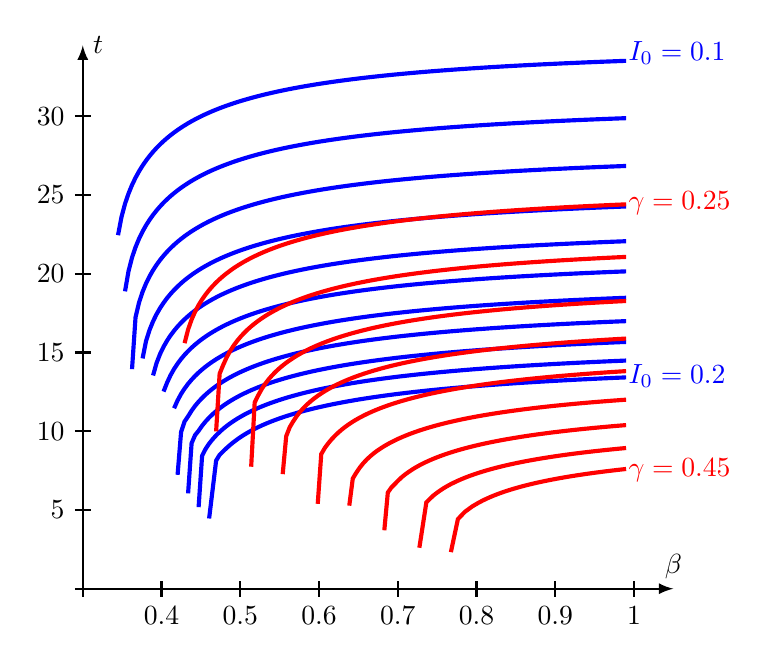
\begin{tikzpicture}[>=latex,thick]

\begin{scope}
\clip (3,0) rectangle (10,7);
\uncover<2->{
\jJ
\jK
\jL
\jM
\jN
\jO
\jP
\jQ
\jR
\jS
\jT
}

\uncover<3->{
%\iA
%\iB
%\iC
%\iD
%\iE
%\iF
%\iG
%\iH
%\iI
\iJ
\iK
\iL
\iM
\iN
\iO
\iP
\iQ
\iR
%\iS
%\iT
}
\end{scope}

\uncover<2->{
\node[color=blue] at ({10-0.2},6.8) [right] {$I_0=0.1$};
\node[color=blue] at ({10-0.2},2.7) [right] {$I_0=0.2$};
}

\uncover<3->{
\node[color=red] at ({10-0.2},4.9) [right] {$\gamma=0.25$};
\node[color=red] at ({10-0.2},1.5) [right] {$\gamma=0.45$};
}

\draw[->] (2.9,0) -- (10.5,0) coordinate[label={$\beta$}];
\draw[->] (3,-0.1) -- (3,6.9) coordinate[label={right:$t$}];

\foreach \b in {4,...,10}{
	\draw ({\b},-0.1)--(\b,0.1);
}
\foreach \t in {5,10,...,30}{
	\draw (2.9,{\t*0.2})--(3.1,{\t*0.2});
}
\node at (2.9,1) [left] {$ 5$};
\node at (2.9,2) [left] {$10$};
\node at (2.9,3) [left] {$15$};
\node at (2.9,4) [left] {$20$};
\node at (2.9,5) [left] {$25$};
\node at (2.9,6) [left] {$30$};

%\node at (3,-0.1) [below] {$0.3$};
\node at (4,-0.1) [below] {$0.4$};
\node at (5,-0.1) [below] {$0.5$};
\node at (6,-0.1) [below] {$0.6$};
\node at (7,-0.1) [below] {$0.7$};
\node at (8,-0.1) [below] {$0.8$};
\node at (9,-0.1) [below] {$0.9$};
\node at (10,-0.1) [below] {$1$};

\end{tikzpicture}
\end{center}
\end{column}
\end{columns}
\end{frame}

\egroup
